\documentclass{tufte-handout}
%\geometry{showframe}% for debugging purposes -- displays the margins

\usepackage{amsmath}

% Set up the images/graphics package
\usepackage{graphicx}
\setkeys{Gin}{width=\linewidth,totalheight=\textheight,keepaspectratio}
\graphicspath{{graphics/}}

\title{Artificial Neural Network and Vacuum Oscillation \thanks{With Shashank}}
\author[Lei Ma]{Lei Ma}
\date{May 01 2015}  % if the \date{} command is left out, the current date will be used

% The following package makes prettier tables.  We're all about the bling!
\usepackage{booktabs}

% The units package provides nice, non-stacked fractions and better spacing
% for units.
\usepackage{units}

% The fancyvrb package lets us customize the formatting of verbatim
% environments.  We use a slightly smaller font.
\usepackage{fancyvrb}
\fvset{fontsize=\normalsize}

% Small sections of multiple columns
\usepackage{multicol}

% code highlighting
\usepackage{listings}

\usepackage{minted}
\usepackage[utf8]{inputenc}
\usepackage[english]{babel}

% Provides paragraphs of dummy text

% These commands are used to pretty-print LaTeX commands
\newcommand{\doccmd}[1]{\texttt{\textbackslash#1}}% command name -- adds backslash automatically
\newcommand{\docopt}[1]{\ensuremath{\langle}\textrm{\textit{#1}}\ensuremath{\rangle}}% optional command argument
\newcommand{\docarg}[1]{\textrm{\textit{#1}}}% (required) command argument
\newenvironment{docspec}{\begin{quote}\noindent}{\end{quote}}% command specification environment
\newcommand{\docenv}[1]{\textsf{#1}}% environment name
\newcommand{\docpkg}[1]{\texttt{#1}}% package name
\newcommand{\doccls}[1]{\texttt{#1}}% document class name
\newcommand{\docclsopt}[1]{\texttt{#1}}% document class option name

\begin{document}

\maketitle% this prints the handout title, author, and date

\begin{abstract}
\noindent This is a summary of the work that has been done on solving vacuum oscillation using artificial neural network. Also included are some tests.
\end{abstract}



The aim of this project is to solve a system that could not be solved using the traditional numerical methods. The system here is a system of neutrinos emitted from a plane but interact with with the neutrinos reflected from some other plane. In this case the evolution of the emitted neutrinos are coupled to itself through the reflection.



\section{Neutrino-neutrino Interaction with The Appearance of Reflection}


Here is the configuration.


\begin{figure}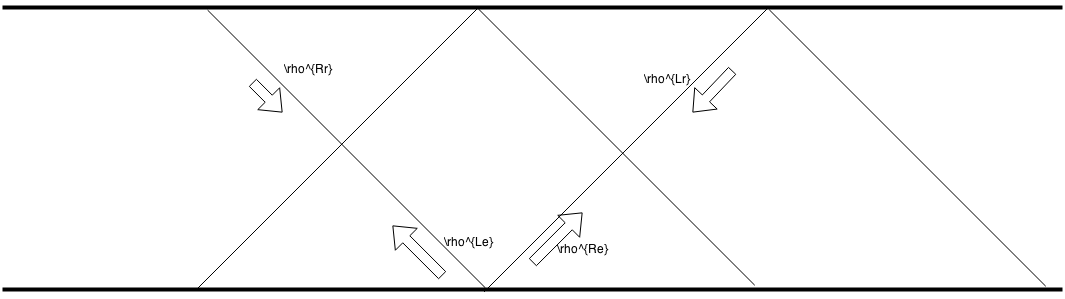
\includegraphics{assets/neutrinoWithReflection}
\caption{Configuration of the system. The lower plane is the emission plane while the upper plane the the reflection plane. Neutrino reaches the upper plane has a probability of being reflected, in other words there is a fixed coefficient for reflection. Only the reflected beams with angle that is the same as the emission angle are considered.}
\end{figure}



The lower plane is the emission plane while the upper plane the the reflection plane. Neutrinos get reflected at the upper plane with a reflection coefficient $\alpha$. The distance between the two plane is $d$.


\begin{marginfigure}[2\baselineskip]
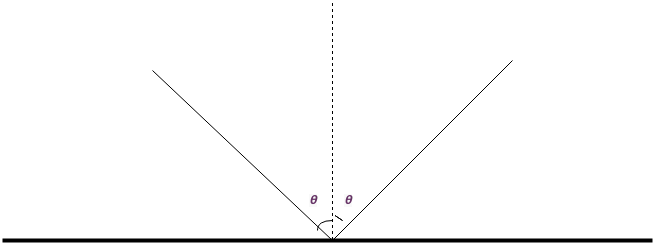
\includegraphics{assets/emissionAngles}
\caption{There is a left-right symmetry of the emission beams. The angles are defined as $\theta$.}
\end{marginfigure}

The notation for neutrino beams are

\begin{itemize}
\item Density Matrix of Emission to The Right:
$\rho^{Re}$
\item Density Matrix of Emission to The Left:
$\rho^{Le}$
\item Density Matrix of Reflection to The Right:
$\rho^{Rr}$
\item Density Matrix of Reflection to The Left:
$\rho^{Lr}$
\item Neutrino-neutrino Interaction of Emission to The Right:
$H_{\nu\nu}^{Re}$
\item Neutrino-neutrino Interaction of Emission to The Left:
$H_{\nu\nu}^{Le}$
\item Neutrino-neutrino Interaction of Reflection to The Right:
$H_{\nu\nu}^{Rr}$
\item Neutrino-neutrino Interaction of Reflection to The Left:
$H_{\nu\nu}^{Lr}$
\end{itemize}





At a fixed, each beam has a neutrino-neutrino interaction Hamiltonian with contribution from another emission beam and two reflected beams.

\begin{marginfigure}[7\baselineskip]
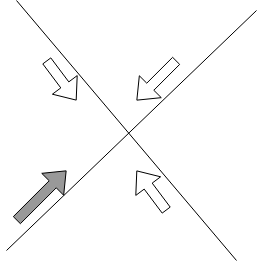
\includegraphics{assets/interactionAtPoint}
\caption{The neutrino-neutrino interaction at a fixed point for a beam going to the right.\newline \textbf{Remake the graph} }
\end{marginfigure}



For a right emission beam, the neutrino-neutrino interaction is



\begin{align}
H_{\nu\nu}^{Re} =& \mu \left( 2 n^{Lr} (\rho^{Lr} -\bar\rho^{Lr}) +  n^{Le}(1-\cos(2\theta) ) (\rho^{Le} -\bar\rho^{Le}) \right. \nonumber \\
& \left. + n^{Rr} (1+\cos(2\theta))(\rho^{Rr} - \bar\rho^{Rr})  \right) 
\end{align}

The equation of motion for this beam is

\begin{align}
i \partial_z \rho^{Re}(z)  = \cos\theta \left[ H_{vac} + H_{\nu\nu}^{Re} ,  \rho^{Re}(z)  \right],
\end{align}

where $\hbar= c =1$.

This equation of motion shows that to calculate the evolution of the density matrix of the emission beam, we need the reflected beam, which, unfortunately depends on the emission beam. This is the reason why we tried artificial neural network.\footnote{However, other methods could be found.}


The other seven equation can also be written down using exactly the same trick. First of all the Hamiltonian are

\begin{align*}
H_{\nu\nu}^{Le} & = \mu \left[ 2 n^{Rr}(\rho^{Rr} - \bar \rho^{Rr}) + n^{Lr}(1+\cos 2\theta )( \rho^{Lr} - \bar \rho^{Lr} )  +  n^{Re} (1-\cos 2\theta) (\rho^{Re} - \bar \rho^{Re})\right] \\
H_{\nu\nu}^{Rr}& = \mu\left[ 2 n^{Le}(\rho^{Le} - \bar \rho^{Le}) + n^{Lr} (1-\cos 2\theta)(\rho^{Lr} - \bar\rho^{Lr}) + n^{Re}(1+\cos 2\theta) (\rho^{Re} - \bar \rho^{Re}) \right] \\
H_{\nu\nu}^{Lr}& = \mu \left[ 2n^{Re}(\rho^{Re}-\bar\rho^{Re}) + n^{Rr} (1-\cos 2\theta) (\rho^{Rr} - \bar \rho^{Rr}) + n^{Le}(1+\cos 2\theta )  (\rho^{Le} - \bar \rho^{Le} ) \right]\\
\end{align*}

The EoMs are


\begin{align}
i\partial_z \rho^{Le}(z) &= \cos\theta \left[ H_{vac} + H_{\nu\nu}^{Le}, \rho^{Le}(z) \right] \\
i\partial_z \rho^{Rr}(z) &= \cos\theta \left[ H_{vac} + H_{\nu\nu}^{Rr}, \rho^{Rr}(z) \right] \\
i\partial_z \rho^{Lr}(z) &= \cos\theta \left[ H_{vac} + H_{\nu\nu}^{Lr}, \rho^{Lr}(z) \right].
\end{align}



For anti-neutrinos, the vacuum Hamiltonian is different from neutrinos which is $\bar H_{vac} = - H_{vac}$. The convention is that $z$ is always pointing up perpendicular to the emission plane.

\begin{align}
- i \partial_z \bar \rho^{Re}(z) & = \cos\theta \left[ \bar H_{vac} + H_{\nu\nu}^{Re} , \bar \rho^{Re}(z)  \right] \\
- i\partial_z \bar\rho^{Le}(z) &= \cos\theta \left[\bar H_{vac} + H_{\nu\nu}^{Le}, \bar\rho^{Le}(z) \right] \\
- i\partial_z \bar\rho^{Rr}(z) &= \cos\theta \left[\bar H_{vac} + H_{\nu\nu}^{Rr}, \bar\rho^{Rr}(z) \right] \\
- i\partial_z \bar \rho^{Lr}(z) &= \cos\theta \left[\bar H_{vac} + H_{\nu\nu}^{Lr}, \bar\rho^{Lr}(z) \right].
\end{align}




To solve the eight first order ODEs, eight constraints are required. To begin with, all the differential equations for the emission beams are given as usual. 

\begin{align}
\rho^{Xe}(z=0) &= \cdots ,
\end{align}

where ${}^{Xe}$ is for ${}^{Le}$ and ${}^{Re}$.

However, the other four constraints are for the reflected beams and they are not clear. \footnote{ {\bf{I have a question here. Since there is no mixing between neutrinos and anti-neutrinos for Dirac particle, I would expect these constraints to be independent of each other. Is this true?}} }

\begin{align}
\rho^{Lr}(z=d) & = \mathbf{Refl} [\rho^{Le}(z=d)] \\
\rho^{Rr}(z=d) & =  \mathbf{Refl} [ \rho^{Rr}(z=d) ]  \\
\bar\rho^{Lr}(z=d) & =  \mathbf{Refl} [\bar \rho^{Le}(z=d)] \\
\bar \rho^{Rr}(z=d) & =  \mathbf{Refl} [ \bar \rho^{Re}(z=d)],
\end{align}

in which $\mathbf{Refl}$ is the operator for the reflection that takes out some of the diagonal elements and multiplied each element by a constant. \footnote{{\bf The question is how to determine this $\mathbf{Refl}$.}}













\section{Artificial Neural Network for Vacuum Oscillation}

To make sure artificial neural network actually works, we started from the calculation of vacuum oscillation. \footnote{In this section we consider only two flavour neutrino oscillation.}


\subsection{Vacuum Oscillation}


Neutrino Vacuum Oscillation is determined by the following equation of motion.

\begin{equation}
i\partial_t \rho = \left[ H_{vac},\rho \right],
\end{equation}

where $\rho$ is the density matrix and can be written as

\begin{equation}
\rho = \begin{pmatrix} a & b + i c\\
b - i c & d \end{pmatrix},
\end{equation}

in which all the $a,b,c,d$ are real.

The vacuum Hamiltonian is

\begin{equation}
H_{vac} = \frac{\delta^2 m}{4 E}\begin{pmatrix} -\cos(2\theta_v) & \sin(2\theta_v)\\
\sin(2\theta_v) & \cos(2\theta_v)\end{pmatrix}.
\end{equation}


Plug in this vacuum Hamiltonian we can write down four equations for $a,b,c,d$. 


Suppose we can write the vacuum Hamiltonian as

\begin{equation}
H_{vac} = \begin{pmatrix} h0 & h1 \\ h2 & h3 \end{pmatrix}.
\end{equation}

Von Neumann equation shows that

\begin{equation}
i \partial_t \rho = \left[ H_{vac}, \rho \right],
\end{equation}

Using the previous notations, I find four equations

\begin{align}
\dot a &= - (h1+h2) c \\
\dot b &= (h0-h3) c \\
\dot c &= a ~ h1 + d~h1 + b (h0-h3) \\
\dot d & = c (h0-h3).
\end{align}



There are two ways of writing the program.

\begin{itemize}
\item 2 by 2 Matrix
\item 1 by 4 Matrix
\end{itemize}



In this note, we will use a 1 by 4 matrix to denote the density matrix, which is defined as,

\begin{equation}
\rho = \begin{pmatrix} a \\ d \\ b \\ c
\end{pmatrix}
\end{equation}

The equation of motion becomes

\begin{align}
\partial_t \begin{pmatrix} a \\ d \\ b \\ c
\end{pmatrix}  = \begin{pmatrix} - (h1+h2) c \\  (h0-h3) c  \\ a~h1 + d~h1 + b (h0-h3) \\ c (h0-h3)  \end{pmatrix}
\end{align}


For vacuum oscillations, the Hamiltonian is

\begin{equation}
H_{vac} \propto = \begin{pmatrix} -\cos 2\theta & \sin 2\theta \\ \sin 2\theta & \cos 2\theta \end{pmatrix},
\end{equation}

which leads to

\begin{equation}
\partial_t \begin{pmatrix} a \\ d \\ b \\ c
\end{pmatrix}  = \begin{pmatrix} - (2 \sin 2\theta ) c \\  -2c \cos 2\theta   \\ a\sin 2\theta + d \sin 2\theta - 2b \cos 2\theta \\ -2c\cos 2\theta   \end{pmatrix}.
\end{equation}


The four equations can be solved and the density matrix at any time can be obtained.





\subsection{Artificial Neural Network for Vacuum Oscillation}


The code I have been testing is written by Shashank for my code doesn't minimized to a good result.But the debugging for my code is also shown below.



\paragraph{Debugging} Compare my code with Shashank's code. 

My code can also be found here at nbviewer:
\url{http://nbviewer.ipython.org/github/NeuPhysics/aNN/blob/master/ipynb/vacOsc4CompSSConvention.ipynb} .



Through the debugging I have confirmed that we have the same function value given the same arguments and the same cost function value in the same condition. But my code doesn't show a good minimization result.


\paragraph{Testing ANN for Vacuum Oscillation using Shashank's Code} These are tests done using Shashank's code. Three types of tests has been done.

{\bf{Using only Nelder-Mead}},

\begin{lstlisting}[language=Python]
vout=minimize(yp,partot,method='Nelder-Mead',tol=1e-11, 
options={"ftol":1e-9, "maxfev": 100000000,"maxiter":1000000000})
\end{lstlisting}

The result appears to be not bad.\footnote{"nfev": number of function evaluation; "nit": number of total iterations.}

\begin{figure}
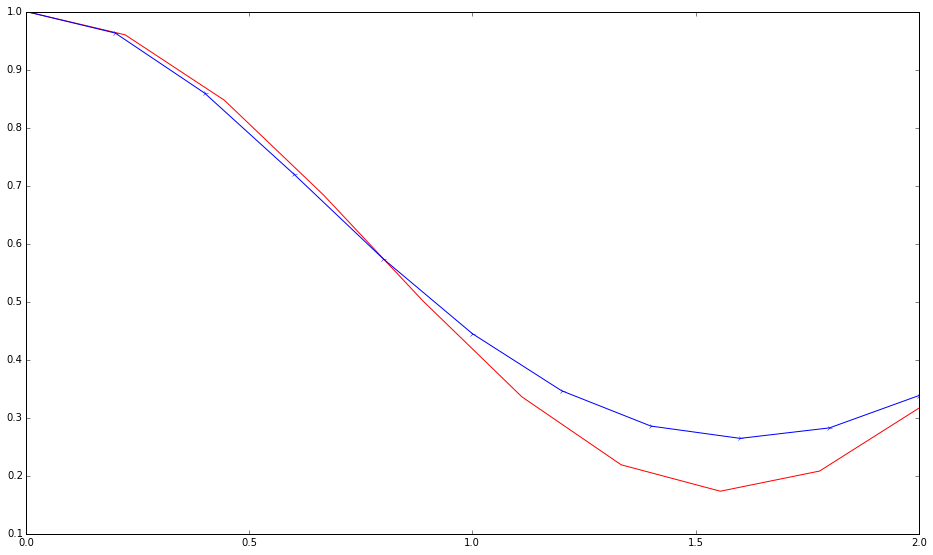
\includegraphics{assets/ann_NelderMead}
\caption{The 11 element of density matrix as a function of time. The red curve is accurate result while the blue is the numerical one.}
\label{fig:ann-NelderMead}
\end{figure}


\begin{verbatim}
status: 0 
nfev: 145333 
success: True 
fun: 0.08876848018538129 
x: array([ 1.21427619, 2.79927002, -0.31095306, -3.03716024, 0.56912385,
0.58925948, -2.20871918, -0.4288958 , -0.32492061, 0.49362869, 0.58244097,
-0.22038025, -0.1011485 , 0.52798698, -2.32437879, 0.44040058, 0.38382487,
0.55826206, -4.94480949, -1.07137694, 4.11333683, -1.50943871, 2.71204262,
-0.76276552, 1.55497648, 0.22475994, 0.88421604, -1.06671129, -2.00532868,
-3.00326507, 0.48030015, 0.25948442, 0.25845743, -0.82423628, 0.78934658,
0.39508506, 0.02805506, -0.02669909, 10.68427395, -1.4504223 , -3.26192936,
7.52701912, -2.55832534, 4.79891183, 4.44328441, -0.14572288, -0.59159877,
0.23857354, -4.99080565, 3.47041765, -2.27428677, -1.07234212, 1.76593101,
-2.21089853, -2.83558577, -0.94328398, -1.99377883, -2.21098883, 0.38034013,
0.43636049]) 
message: 'Optimization terminated successfully.' 
nit: 131078
\end{verbatim}







{\bf{Using Only Differential Evolution}}

For a range of time in (0,2),
\begin{verbatim}
x=np.linspace(0,2,11)
\end{verbatim}

and using only differential evolution,
\begin{verbatim}
vout=differential_evolution(yp,bounds,strategy='best1bin',tol=0.1,
maxiter=100, polish=True)
\end{verbatim}

the function result turns out to be,
\begin{verbatim}
5.649973778537050774e-03
\end{verbatim}

while the result for x array is
\begin{verbatim}
[-0.46752427 -2.65884641 -0.87100392 2.21847349 -0.68876981
-1.18718098 -2.45899394 -2.41608376 -2.03016303 -2.50621246
-1.72752687 -3.52288081 4.53627758 -0.11251283 -2.78713549
-0.44748985 1.64193553 -0.92174658 -0.99302148 1.09775197
-1.17935884 -1.71925608 -2.83591163 -0.52258003 -2.71429398
1.35386314 3.34156037 0.96810593 0.24346204 -4.39480932 2.09637481
-0.74179975 3.26104658 -2.72595898 -0.76631589 -2.21640847
-3.25833908 -0.78663055 -1.55206952 0.46654166 -4.8803229
-4.26865044 -0.12565569 0.10469799 -1.8695357 -0.15555892
-1.17371098 0.26577405 0.875804 -2.51542228 -4.29488662 -2.6605975
1.96894693 -3.09901811 -1.39401083 0.96014599 2.95403418
3.79841345 -2.10529717 -4.10821308]
\end{verbatim}



\begin{figure}
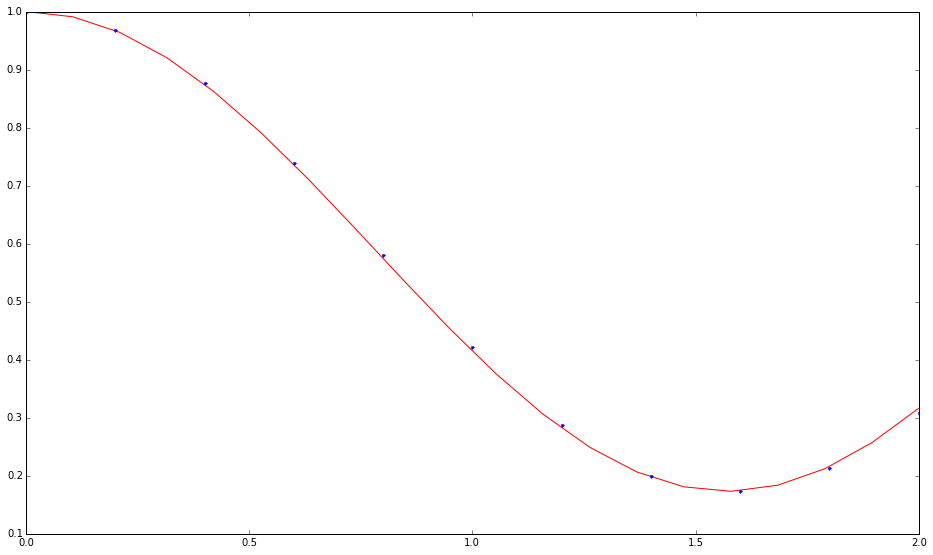
\includegraphics{assets/ann_devo}
\caption{The 11 element of density matrix as a function of time. The red curve is accurate result while the blue is from differential evolution.}
\label{fig:ann-DEvo}
\end{figure}




{\bf{Calculating a Longer Range}}

Double the range to

\begin{verbatim}
x=np.linspace(0,4,11)
\end{verbatim}

and apply only differential evolution.

\begin{verbatim}
vout=differential_evolution(yp,bounds,strategy='best1bin',tol=0.01, maxiter=1000,polish=True)
\end{verbatim}

The result is very bad.

\begin{verbatim}
nfev: 105906 
success: False 
fun: 0.15264565359933352 
x: array([ 1.2415797 , -1.27267036, 0.14521048, 1.06534837, -0.22554095,
1.97210186, 4.85844909, -1.5015446 , -2.66713337, -0.59127114, -1.17100097,
0.72691612, -3.84768313, 0.68169926, 1.61422628, -1.69251485, 0.61827763,
-1.70389394, -2.90578576, 4.69827117, -4.18291259, -1.74349331, 3.76258326,
0.95722587, 5. , 2.80036916, -4.24126024, -2.45899517, 0.99396641, 1.54324845,
-2.99045871, -0.26770419, 1.62076744, -3.41084945, -1.31280928, -2.21778869,
2.4837208 , 2.81803398, -3.94093507, 1.63757038, -3.5154411 , 2.93116174,
0.74082291, -3.26617915, -0.19332002, 1.75131816, -1.46409058, 2.342905 ,
-1.78805522, -2.55208371, -3.55389878, -3.7073305 , -1.98135275, -3.88337902,
-3.3127076 , 0.13548304, 1.90006674, -3.89693459, -1.37139011, -2.28290761])
message: 'Maximum number of iterations has been exceeded.' 
jac: array([ 9.90042492e-02, 9.56093427e-02, 5.69877479e-05, 9.94637706e-04,
3.43239936e-02, 4.57047178e-03, -1.29582733e-03, 2.14828155e-06,
-4.48536763e-03, -1.63860814e-02, -2.19701479e-03, -4.18309276e-03,
8.10185252e-06, -4.03330425e-03, -4.40266712e-03, -9.43032319e-03,
-1.44689816e-04, -1.15090820e-01, -1.20024951e-01, -1.24700941e-01,
-1.07455711e-03, -1.56707980e-05, -3.08311154e-03, 2.43753712e-02,
-3.95701805e-03, -5.22216714e-03, -8.87512286e-05, -5.17548226e-03,
1.23602240e-02, -4.17025858e-03, 4.53925786e-04, -6.57369575e-02,
-6.92782415e-02, 4.67753614e-04, -7.70130126e-02, -3.59692831e-04,
-5.45286039e-05, 3.42913198e-03, 1.46133106e-04, 7.60768115e-03,
-1.32331091e-03, -1.87794225e-04, 5.21242494e-03, -1.47535317e-03,
-8.97968366e-03, 3.09193504e-03, -7.49011964e-05, -2.00667261e-04,
1.80120363e-03, 7.68457520e-04, -2.31557273e-03, -1.89914195e-03,
-2.09954831e-03, 6.48930909e-04, 7.02615743e-04, 4.39465131e-04,
4.34813574e-03, -4.79563611e-04, -2.18436380e-03, -1.66073266e-03]) 
nit: 100
\end{verbatim}




\begin{figure}
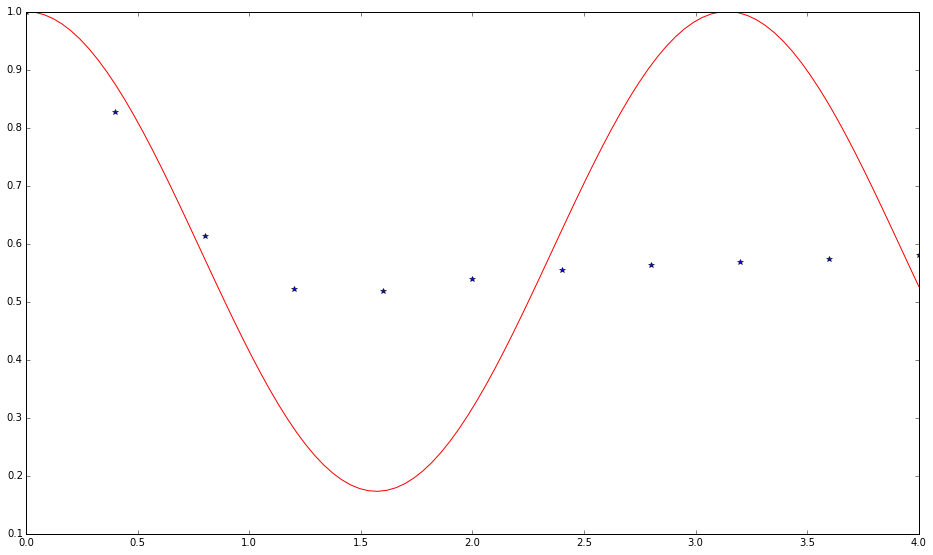
\includegraphics{assets/ann_devo_range}
\caption{The 11 element of density matrix as a function of time. The red curve is accurate result while the blue is from differential evolution.}
\label{fig:ann-DEvo}
\end{figure}






\section{Codes}



\begin{lstlisting}[language=Python]
import numpy as np
from scipy.optimize import minimize
from scipy.special import expit
import matplotlib.pyplot as plt
import scipy
from matplotlib.lines import Line2D
import timeit
import pandas as pd

array12 = np.asarray(np.split(np.random.rand(1,60)[0],12))

def act(x):
    return expit(x)


# Density matrix in the forms that I wrote down on my Neutrino Physics notebook
# x is a real array of 12 arrays.

init = np.array([1.0,0.0,0.0,0.0])

def rho(x,ti,initialCondition):

    elem = np.ones(4)

    for i in np.linspace(0,3,4):
        elem[i] = np.sum(ti*x[i*3]*act(ti*x[i*3+1] + x[i*3+2]) )

    return init + elem


rho(array12,0,init)


hamil = np.array( [  np.cos(2.0),np.sin(2.0) , np.sin(2.0),np.cos(2.0) ] )
print hamil


def rhop(x,ti,initialCondition):

    rhoprime = np.zeros(4)

    for i in np.linspace(0,3,4):
        rhoprime[i] = np.sum(x[i*3] * (act(ti*x[i*3+1] + x[i*3+2]) ) ) +  np.sum( ti*x[i*3]* (act(ti*x[i*3+1] + x[i*3+2]) ) * (1.0 - (act(ti*x[i*3+1] + x[i*3+2])  ) )* x[i*3+1]  )

    return rhoprime



## This is the regularization which is not used in this code

regularization = 0.0001

def costi(x,ti,initialCondition):

    rhoi = rho(x,ti,initialCondition)
    rhopi = rhop(x,ti,initialCondition)

    costTemp = np.zeros(4)

    costTemp[0] = ( rhopi[0] - 2.0*rhoi[3]*hamil[1] )**2
    costTemp[1] = ( rhopi[1] + 2.0*rhoi[3]*hamil[1] )**2
    costTemp[2] = ( rhopi[2] - 2.0*rhoi[3]*hamil[0] )**2
    costTemp[3] = ( rhopi[3] + 2.0*rhoi[2]*hamil[0] - hamil[1] * (rhoi[1] - rhoi[0] ) )**2

    return np.sum(costTemp)# + 2.0*(rhoi[0]+rhoi[1]-1.0)**2


#    return np.sum(costTemp) + regularization*np.sum(x**2)


costi(array12,0,init)

def cost(x,t,initialCondition):

    costTotal = map(lambda t: costi(x,t,initialCondition),t)

    return 0.5*np.sum(costTotal)


cost(array12,np.array([0,1,2]),init)
#cost(xresult,np.array([0,4,11]),init)

# initGuess = np.asarray(np.split( 5.0*(np.random.rand(1,60)[0] - 0.5),12))
initGuess = np.split(np.zeros(60),12)
endpoint = 2
tlin = np.linspace(0,endpoint,11)

costF = lambda x: cost(x,tlin,init)

start = timeit.default_timer()
costvFResult = minimize(costF,initGuess,method='Nelder-Mead',tol=1e-5,options={"ftol":1e-3, "maxfev": 10000000,"maxiter":10000000})
stop = timeit.default_timer()

print stop - start
timespent = stop - start

print costvFResult



xresult = costvFResult.get("x")

print xresult

#np.savetxt('costvFResult.txt',costvFResult,delimiter=',')

np.savetxt('xresult.txt', xresult, delimiter = ',')

np.savetxt('timespent.txt', np.array([timespent]), delimiter = ',')

np.savetxt('functionvalue.txt', np.array([costvFResult.fun]), delimiter=',')

\end{lstlisting}







\end{document}
